\documentclass{article}


\usepackage[a4paper]{geometry}
\usepackage{pgfplots}
\pgfplotsset{compat=1.9}


\usepackage{parskip}


\usepackage[justification=centering]{caption}
\usepackage{subcaption}
\usepackage{graphicx}
\usepackage{float}
\usepackage{amsmath}
\usepackage{booktabs}
\usepackage{tabularx}
\usepackage{perpage}
\usepackage{smartdiagram}
\usepackage{cancel}
\usepackage{amssymb}
\usepackage{bm}
\usepackage{longtable}
\usepackage{listings}
\usepackage{courier}
\usepackage{fancybox}
\newcolumntype{P}[1]{>{\centering\arraybackslash}p{#1}}
\usepackage{hhline}
\usepackage{bm}
\usepackage{siunitx}
\usepackage[utf8]{inputenc}
\usepackage[english]{babel}
\usepackage{graphicx}
\usepackage{amsthm}
\usepackage{tabularray}
\usepackage{verbatim}
\usepackage{verbatimbox}
\usepackage{array}
\usepackage{ulem}
\usepackage{mathtools}
\usepackage{amsfonts}

\usepackage{color}

\usepackage{xparse}




\usepackage{tikz}
\usetikzlibrary{calc}
\usetikzlibrary{automata}
\usetikzlibrary{backgrounds}
\usetikzlibrary{fit}
\usetikzlibrary{arrows}
\usetikzlibrary{arrows.meta}
\usetikzlibrary{decorations.pathreplacing}
\usetikzlibrary{decorations.markings}
\usetikzlibrary{positioning}
\usetikzlibrary{intersections}
\usetikzlibrary{calligraphy}
\usetikzlibrary{patterns}
\usetikzlibrary{shapes}
\usetikzlibrary{shapes.geometric}
\usetikzlibrary{shadows}
\usetikzlibrary{fadings}
\usetikzlibrary{backgrounds}
\usepgflibrary{shadings}


\tikzset{
    loop above right/.style={above right, out= 60, in= 30, loop},
    loop above left/.style ={above left,  out=150, in=120, loop},
    loop below right/.style={below right, out=330, in=300, loop},
    loop below left/.style ={below left,  out=240, in=210, loop}
}

\renewcommand{\thefootnote}{\fnsymbol{footnote}}
\MakePerPage{footnote}


\newtheorem{theorem}{Theorem}[section]
\newtheorem*{theorem*}{Theorem}
\newtheorem{corollary}{Corollary}[theorem]
\newtheorem*{corollary*}{Corollary}
\newtheorem{lemma}[theorem]{Lemma}
\newtheorem*{lemma*}{Lemma}


\newtheorem*{claim}{Claim}

\theoremstyle{definition}
\newtheorem*{proposition}{Proposition}

\theoremstyle{definition}
\newtheorem{definition}{Definition}[section]

\theoremstyle{remark}
\newtheorem*{remark}{Remark}
\newtheorem*{example}{Example}

\renewcommand\qedsymbol{$\blacksquare$}

\usepackage[myheadings]{fullpage}
\usepackage{fancyhdr}
\usepackage{lastpage}
\usepackage{float}
\usepackage{url}
\usepackage{lipsum}
\usepackage[T1]{fontenc}
\usepackage{icomma}
\usepackage{siunitx}
\usepackage{ragged2e}
\usepackage{comment}
\usepackage{multicol}
\usepackage{caption}
\usepackage{float}
\usepackage{titling}
\usepackage{blindtext}
\usepackage{mathdots}
\usepackage{enumitem}
\usepackage{adjustbox}
\usepackage{colortbl}

\pagestyle{fancy}
%\renewcommand{\chaptername}{}
%\renewcommand{\chaptermark}[1]{\markboth{#1}{}}
\renewcommand{\sectionmark}[1]{\markright{#1}{}}
%\renewcommand{\subsectionmark}[1]{\markright{#1}{}}

\fancyhf{}
\setlength\headheight{15pt}
\fancyhead[L]{Tikz/PGF} %>>>MODULE CODE
\fancyhead[R]{reeeeeee} %>>>MODULE NAME
\fancyfoot[C]{Bottom text | \thepage}

\fancypagestyle{plain}{%
    \fancyhf{}%
    \renewcommand{\headrulewidth}{0pt}% 
}

\frenchspacing
\usepackage{bigfoot}
\renewcommand{\footnoterule}{\vfill\kern -3pt \hrule width 0.4\columnwidth \kern 2.6pt}



\newcommand{\Tikz}{Ti\textit{k}z{}}


\begin{document}

\title{Introduction to PGF/\Tikz{}}

\newpage

\section*{What is PGF/\Tikz{}?}

PGF/\Tikz{} is a pair of languages for generating \textit{vector graphics}. That is, graphics constructed from geometric primitives (points/vertices, line segments, polyhedra, parametric surfaces, etc.), with each primitive assigned a set of properties (colour, line weight, dash patterns, etc.). This is in contrast to \textit{raster graphics}, in which each pixel of the image is stored (e.g. with colour, luminance, transparency values, etc.).

Because vector graphics consist of coordinates/lines/curves, the size of a representation on a screen is independent of the size of the object -- you can zoom in to a vector image arbitrarily close and it will remain crisp.

Furthermore, the parameters of vector objects can be later modified, so that moving, scaling, rotating, filling, etc. does not degrade the quality of a vector image. In contrast, repeated modifications to a raster image will continually degrade the image quality as elements are snapped to a pixel grid between each edit.

\section*{Getting Started}

A \Tikz{} diagram is built within the \verb|tikzpicture| environment. Primitives are specified and drawn using \Tikz{} commands within the environment, each terminated with a semicolon (\verb|;|).

Here is an example of some \Tikz{} code, and its output:


\subsection*{Specifying Points}

There are many ways to specify \textit{points} or \textit{coordinates} in \Tikz{}. You can declare your coordinate system explicitly (this will be more relevant later) with the syntax
\begin{verbatim}
    ([coordinate system] cs: (system-specific coordinates))
\end{verbatim}
but for various common coordinate systems, special implicit syntax is available.

For instance, cartesian coordinate may be specified explicitly using the \verb|canvas| coordinate system:
\begin{verbatim}
    (canvas cs:x=2ex,y=5pt)
\end{verbatim}
which takes two keys, \verb|x| and \verb|y|, that accept \TeX{} dimensions. Or, they can be specified implicitly by listing the two dimensions separated by commas in round brackets, as in
\begin{verbatim}
    (2ex,5pt)
\end{verbatim}
This coordinate means ``2ex upwards and 5pt to the right of the origin''.

Note that you can also write things like \verb|1em+2cm| in a dimension, since the maths engine is used to evaluate the coordinates.

\begin{verbbox}[\small\mbox{}]
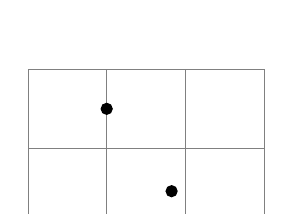
\begin{tikzpicture}
    \draw[help lines] (0,0) grid (3,2);

    \filldraw (1cm,1.5cm)   circle (2pt);
    \filldraw (2cm-5pt,3ex) circle (2pt);
\end{tikzpicture}
\end{verbbox}
\begin{center}
    $\vcenter{\hbox{
    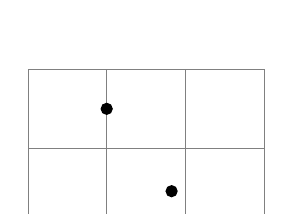
\begin{tikzpicture}
        \draw[help lines] (0,0) grid (3,2);
    
        \filldraw (1cm,1.5cm)   circle (2pt);
        \filldraw (2cm-5pt,3ex) circle (2pt);
    \end{tikzpicture}
    }}$
    \hspace*{0.5cm}
    $\vcenter{\hbox{\theverbbox}}$
\end{center}

Polar coordinates may be specified using the \verb|canvas polar| system
\begin{verbatim}
    (canvas polar cs:angle=30,radius=2cm)
\end{verbatim}
or implicitly by providing the angle and a radius separated by a colon:
\begin{verbatim}
    (30:2cm)
\end{verbatim}
This coordinate means ``2cm from the origin, 30 degrees counterclockwise from the positive $x$-axis''.

\begin{verbbox}[\small\mbox{}]
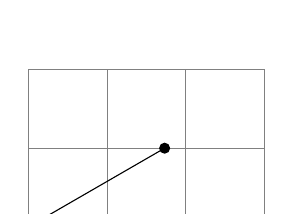
\begin{tikzpicture}
    \draw[help lines] (0,0) grid (3,2);
    \draw (0,0) -- (30:2cm);

    \fill (30:2cm) circle (2pt);
\end{tikzpicture}
\end{verbbox}
\begin{center}
    $\vcenter{\hbox{
    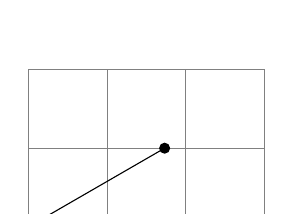
\begin{tikzpicture}
        \draw[help lines] (0,0) grid (3,2);
        \draw (0,0) -- (30:2cm);
    
        \fill (30:2cm) circle (2pt);
    \end{tikzpicture}
    }}$
    \hspace*{0.5cm}
    $\vcenter{\hbox{\theverbbox}}$
\end{center}

There are other coordinate systems, but we'll only discuss those on request. From now on, we'll also omit the explicit system declaration unless it is otherwise relevant.

If units are not provided, e.g. \verb|(1,2)|, then the coordinates are specified in PGF's internal \verb|xy|-coordinate system. By default, the unit $x$-vector points 1cm to the right, and the unit $y$-vector points 1cm upwards.\footnote{It is possible to use coordinates like \verb|(1,2cm)|, which is neither an \verb|xy|-coordinate nor a \verb|canvas| coordinate. Roughly speaking, if you have mixed coordinates, \Tikz{} will typecast the coordinate \verb|(X,Ycm)| to the sum \verb|(X,0)+(0pt,Y)|, and similarly for any mixed dimensions. In particular, \verb|(2+3cm,0)| is \textit{not} the same as \verb|(2cm+3cm,0)|, as it will be typecast to the sum \verb|(2pt,0) + (3cm,0) = (2pt+3cm,0)|.}

By giving three numbers, as in \verb|(1,2,3)|, the coordinates are specified in PGF's internal $xyz$-coordinate system. By default, the unit $x$-vector points 1cm to the right, and the unit $y$-vector points 1cm upwards, and the unit $z$-vector points to \verb|(-3.85mm,-3.85mm)|.

It is also possible to use an anchor (explained later) of an existing shape as in \verb|(my\_node.centre)| as a coordinate.

You can add two plus signs before a coordinate to specify a coordinate relative to the previously defined coordinate. For example, \verb|(1,0) ++(1,0) ++(0,1)| specifies the three coordinates \verb|(1,0)|, then \verb|(2,0)|[=(1,0)+(1,0)], and \verb|(2,1)|[$=(2,0)+(0,1)$].

Instead of two plus signs, you can also add a single one. This also specifies a point in a relative manner, but doesn't update the reference coordinate. For example, \verb|(1,0) +(1,0) +(0,1)| specifies the three coordinates \verb|(1,0)|, then \verb|(2,0)|[$=(1,0)+(1,0)$], and \verb|(1,1)|[$=(1,0)+(0,1)$].






\subsection*{Paths}

A \textit{path} is a series of curves between points, which need not be connected.

To specify a straight line path between two coordinates, put two dashes between the coordinates. For instance,
\begin{verbatim}
    (0,0) -- (0,1) -- (1,1) -- cycle
\end{verbatim}
specifies a trianglar path, with the special \verb|cycle| coordinate \textit{smoothly} closing the path. To see the difference between using \verb|cycle| and simply repeating the first coordinate, consider the following:
\begin{verbbox}[\small\mbox{}]

\begin{tikzpicture}[line width=5pt]
    \path[draw] (0,0) -- (0,1) -- (1,1) -- cycle;
    \path[draw] (2,0) -- (2,1) -- (3,1) -- (2,0);
\end{tikzpicture}
\end{verbbox}
\begin{center}
    $\vcenter{\hbox{
    
\begin{tikzpicture}[line width=5pt]
        \draw (0,0) -- (0,1) -- (1,1) -- cycle;
        \draw (2,0) -- (2,1) -- (3,1) -- (2,0);
    \end{tikzpicture}
    }}$
    \hspace*{0.5cm}
    $\vcenter{\hbox{\theverbbox}}$
\end{center}

\subsection*{Shapes and Special Paths}

There are various commands for generating predefined shapes and patterns. For instance,
\begin{verbatim}
    (a,b) rectangle (c,d)
\end{verbatim}
specifies a rectangular box with opposite corners at \verb|(a,b)| and \verb|(c,d)|.
\begin{verbbox}[\small\mbox{}]
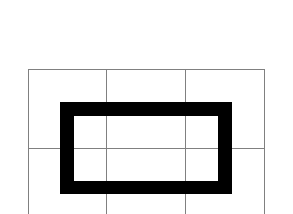
\begin{tikzpicture}[line width=5pt]
    \draw[help lines] (0,0) grid (3,2);

    \path[draw] (0.5,0.5) rectangle (2.5,1.5);
\end{tikzpicture}
\end{verbbox}
\begin{center}
    $\vcenter{\hbox{
    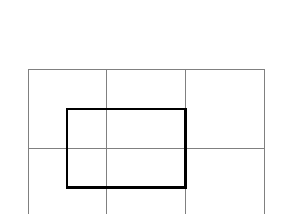
\begin{tikzpicture}
        \draw[help lines] (0,0) grid (3,2);
        
        \draw[thick] (0.5,0.5) rectangle (2,1.5);
    \end{tikzpicture}
    }}$
    \hspace*{0.5cm}
    $\vcenter{\hbox{\theverbbox}}$
\end{center}

\begin{verbatim}
    (a,b) circle (r)
\end{verbatim}
specifies a circle centred at \verb|(a,b)| with radius \verb|r|.
\begin{verbbox}[\small\mbox{}]
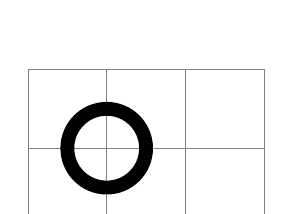
\begin{tikzpicture}[line width=5pt]
    \draw[help lines] (0,0) grid (3,2);
    
    \path[draw] (1,1) circle (0.5);
\end{tikzpicture}
\end{verbbox}
\begin{center}
    $\vcenter{\hbox{
    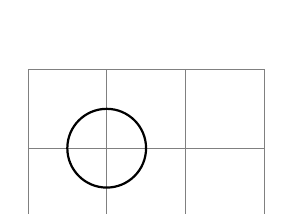
\begin{tikzpicture}
        \draw[help lines] (0,0) grid (3,2);
        
        \draw[thick] (1,1) circle (0.5);
    \end{tikzpicture}
    }}$
    \hspace*{0.5cm}
    $\vcenter{\hbox{\theverbbox}}$
\end{center}




\subsection*{Actions}

Note that, so far, a path is simply a series of curves and coordinates -- we haven't actually told \Tikz{} what to do with them.

Given a path, we may:
\begin{itemize}
    \item \textit{draw} or \textit{stroke} the path;
    \item \textit{fill} the path;
    \item \textit{clip} the path;
    \item (various other specialised options);
    \item or do any combination of the above.
\end{itemize}

To perform these actions, pass them as options to the \verb|\path| command or use one of these aliases:
\begin{verbatim}
    \draw ...     := \path[draw] ...
    \fill ...     := \path[fill] ...
    \filldraw ... := \path[fill,draw] ...
    etc.
\end{verbatim}

\bigbreak

\begin{verbbox}[\small\mbox{}]

\begin{tikzpicture}
    \path     (0,0) circle (0.5); % does nothing
    \draw     (2,0) circle (0.5);
    \fill     (4,0) circle (0.5);
\end{tikzpicture}
\end{verbbox}
\begin{center}
    $\vcenter{\hbox{
        
\begin{tikzpicture}
            \path     (0,0) circle (0.5); % does nothing
            \draw     (2,0) circle (0.5);
            \fill     (4,0) circle (0.5);
        \end{tikzpicture}
    }}$
    \hspace*{0.5cm}
    $\vcenter{\hbox{\theverbbox}}$
\end{center}

There are many other options you can pass to a draw command, but some important ones include:
\begin{itemize}
    \item colours;
    \item opacities;
    \item stroke width;
    \item dash patterns;
    \item arrow tips.
\end{itemize}

Passing a colour to a \verb|\draw| command will set the global colour in that scope, so all lines, fills, labels, etc. will all use that colour unless overridden locally. (Opacity has a similar discussion.) If any options are unset, they will default to black/full opacity (defaults may also be modified).

More specialised options that only set individual colours/opacities may also be used:
\begin{verbbox}[\small\mbox{}]
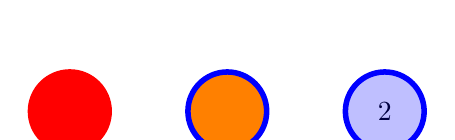
\begin{tikzpicture}[line width=2pt]
    \draw (2,0) node {$1$} (4,0) node {$2$};

    \filldraw[red]                    (0,0) circle (0.5);
    \filldraw[draw=blue,fill=orange]  (2,0) circle (0.5);
    \filldraw[blue,fill opacity=0.25] (4,0) circle (0.5);
\end{tikzpicture}
\end{verbbox}
\begin{center}
    $\vcenter{\hbox{
    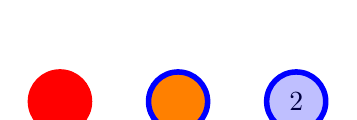
\begin{tikzpicture}[line width=2pt,scale=0.75]
        \draw (2,0) node {$1$} (4,0) node {$2$};

        \filldraw[red]                    (0,0) circle (0.5);
        \filldraw[draw=blue,fill=orange]  (2,0) circle (0.5);
        \filldraw[blue,fill opacity=0.25] (4,0) circle (0.5);
    \end{tikzpicture}
    }}$
    $\vcenter{\hbox{\theverbbox}}$
\end{center}

Sidenote on opacity and drawing precedence: \Tikz{} draws objects on top of each other, in the order they are given. So, if you want something to appear behind something else, the obscured object must be drawn first, i.e. above the line where the obscuring object is drawn.

As well as passing options to individual \verb|\draw| commands, you can pass options to the environment to set that option globally for everything in that environment. For instance, the \verb|line width| option for all the draw commands is set to \verb|2pt| at the top, so we don't need to set it for each draw command individually.

Stroke widths affect the width of the paths drawn, and can be set with. There are various built-in widths available:
\begin{verbbox}[\small\mbox{}]
    
\begin{tikzpicture}[yscale=0.4]
        \draw[ultra thin]  (0,6) -- (3,6);
        \draw[very thin]   (0,5) -- (3,5);
        \draw[thin]        (0,4) -- (3,4);
        \draw[semithick]   (0,3) -- (3,3);
        \draw[thick]       (0,2) -- (3,2);
        \draw[very thick]  (0,1) -- (3,1);
        \draw[ultra thick] (0,0) -- (3,0);
    \end{tikzpicture}
\end{verbbox}
\begin{center}
    $\vcenter{\hbox{
    
\begin{tikzpicture}[yscale=0.4]
        \draw[ultra thin]  (0,6) -- (3,6);
        \draw[very thin]   (0,5) -- (3,5);
        \draw[thin]        (0,4) -- (3,4);
        \draw[semithick]   (0,3) -- (3,3);
        \draw[thick]       (0,2) -- (3,2);
        \draw[very thick]  (0,1) -- (3,1);
        \draw[ultra thick] (0,0) -- (3,0);
    \end{tikzpicture}
    }}$
    $\vcenter{\hbox{\theverbbox}}$
\end{center}
Arrows can also be added using this syntax:
\begin{verbatim}
    \draw[->] ...
\end{verbatim}
or similar. There are also various types of arrowheads, \verb|>| being one of the basic kinds. More configurations are listed below:
\begin{verbbox}[\small\mbox{}]
    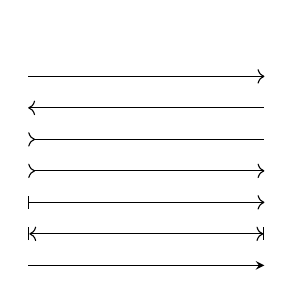
\begin{tikzpicture}[yscale=0.4]
        \draw[->]                   (0,7) -- (3,7);
        \draw[<-]                   (0,6) -- (3,6);
        \draw[>-]                   (0,5) -- (3,5);
        \draw[>->]                  (0,4) -- (3,4);
        \draw[|->]                  (0,3) -- (3,3);
        \draw[|<->|]                (0,2) -- (3,2);
        \draw[-stealth]             (0,1) -- (3,1);
        \draw[-latex]               (0,0) -- (3,0);
    \end{tikzpicture}
\end{verbbox}
\begin{center}
    $\vcenter{\hbox{
    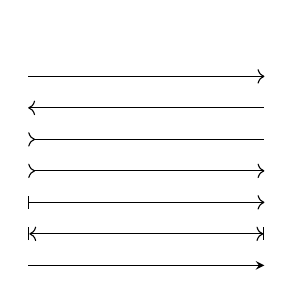
\begin{tikzpicture}[yscale=0.4]
        \draw[->]                   (0,7) -- (3,7);
        \draw[<-]                   (0,6) -- (3,6);
        \draw[>-]                   (0,5) -- (3,5);
        \draw[>->]                  (0,4) -- (3,4);
        \draw[|->]                  (0,3) -- (3,3);
        \draw[|<->|]                (0,2) -- (3,2);
        \draw[-stealth]             (0,1) -- (3,1);
        \draw[-latex]               (0,0) -- (3,0);
    \end{tikzpicture}
    }}$
    $\vcenter{\hbox{\theverbbox}}$
\end{center}
Other usual options may also be passed locally to the arrowhead:
\begin{verbbox}[\small\mbox{}]
    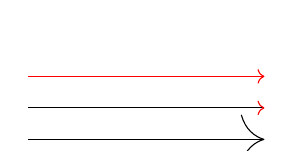
\begin{tikzpicture}[yscale=0.4]
        \draw[red,->]           (0,2) -- (3,2);
        \draw[-{>[red]}]        (0,1) -- (3,1);
        \draw[-{>[length=3mm]}] (0,0) -- (3,0);
    \end{tikzpicture}
\end{verbbox}
\begin{center}
    $\vcenter{\hbox{
    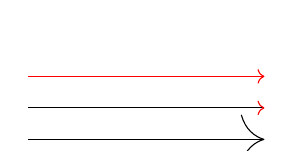
\begin{tikzpicture}[yscale=0.4]
        \draw[red,->]           (0,2) -- (3,2);
        \draw[-{>[red]}]        (0,1) -- (3,1);
        \draw[-{>[length=3mm]}] (0,0) -- (3,0);
    \end{tikzpicture}
    }}$
    $\vcenter{\hbox{\theverbbox}}$
\end{center}
Lines can also be dashed/dotted. There are various built-in pattern available (not all listed):
\begin{verbbox}[\small\mbox{}]
    \begin{tikzpicture}[yscale=0.4]
        \draw[dotted]         (0,6) -- (3,6);
        \draw[densely dotted] (0,5) -- (3,5);
        \draw[loosely dotted] (0,4) -- (3,4);
        \draw[dashed]         (0,3) -- (3,3);
        \draw[densely dashed] (0,2) -- (3,2);
        \draw[loosely dashed] (0,1) -- (3,1);
        \draw[dash dot]       (0,0) -- (3,0);
    \end{tikzpicture}
\end{verbbox}
\begin{center}
    $\vcenter{\hbox{
    \begin{tikzpicture}[yscale=0.4]
        \draw[dotted]         (0,6) -- (3,6);
        \draw[densely dotted] (0,5) -- (3,5);
        \draw[loosely dotted] (0,4) -- (3,4);
        \draw[dashed]         (0,3) -- (3,3);
        \draw[densely dashed] (0,2) -- (3,2);
        \draw[loosely dashed] (0,1) -- (3,1);
        \draw[dash dot]       (0,0) -- (3,0);
    \end{tikzpicture}
    }}$
    $\vcenter{\hbox{\theverbbox}}$
\end{center}
More generally, you can specify the pattern manually using the \verb|dash pattern| option:
\begin{verbatim}
    dash pattern=x on y off
\end{verbatim}
where \verb|x| and \verb|y| are any \TeX{} dimensions.


\subsection*{Nodes}



\subsection*{The Calc Library}



\section*{Your First \Tikz{} Diagram}






\section*{Anchors}

\tikzset{
    shape example/.style= {color = black!30,
                           draw,
                           fill = yellow!30,
                           line width = .5cm,
                           inner xsep = 2.5cm,
                           inner ysep = 0.5cm}
}

\begin{center}
    \begin{tikzpicture}
        \node[name=s,shape=circle,shape example] {Circle\vrule width 1pt height 2cm};
        \foreach \anchor/\placement in
            {north west/above left, north/above, north east/above right,
            west/left, center/above, east/right,
            mid west/right, mid/above, mid east/left,
            base west/left, base/below, base east/right,
            south west/below left, south/below, south east/below right,
            text/left, 10/right, 130/above}
            \draw[shift=(s.\anchor)] plot[mark=x] coordinates{(0,0)}
                node[\placement] {\scriptsize\texttt{(s.\anchor)}};
    \end{tikzpicture}
\end{center}

\begin{center}
    \begin{tikzpicture}
        \node[name=s,shape=rectangle,shape example] {Rectangle\vrule width 1pt height 2cm};
        \foreach \anchor/\placement in
            {north west/above left, north/above, north east/above right,
            west/left, center/above, east/right,
            mid west/right, mid/above, mid east/left,
            base west/left, base/below, base east/right,
            south west/below left, south/below, south east/below right,
            text/left, 10/right, 130/above}
            \draw[shift=(s.\anchor)] plot[mark=x] coordinates{(0,0)}
                node[\placement] {\scriptsize\texttt{(s.\anchor)}};
    \end{tikzpicture}
\end{center}










\newpage
\section*{Samples}

\subsection*{Iteration}

\begin{center}
    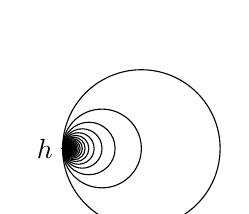
\begin{tikzpicture}
        \foreach \n in {1,...,100}
            \draw[thin] (1/\n,0) circle (1/\n);
        \draw (0,0) node [left] {$h$};
    \end{tikzpicture}
\end{center}

\vspace*{2cm}

\begin{center}
    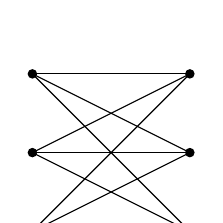
\begin{tikzpicture}
        \foreach \l in {0,1,2} {
            \foreach \r in {0,1,2} {
                \draw (0,2\l) -- (2,2\r);
            }
            \filldraw (0,2\l) circle (1.5pt);
            \filldraw (2,2\l) circle (1.5pt);
        }
    \end{tikzpicture}
\end{center}

\vspace*{2cm}

\begin{equation*}
    Z=\{0\}\cup\textcolor{blue}{\{2^{-n}:n\in\mathbb{Z}^+\}}\cup\textcolor{cyan}{\{2^{-n}+2^{-n-m}:n,m\in\mathbb{Z}^+\}}
\end{equation*}

\begin{center}
    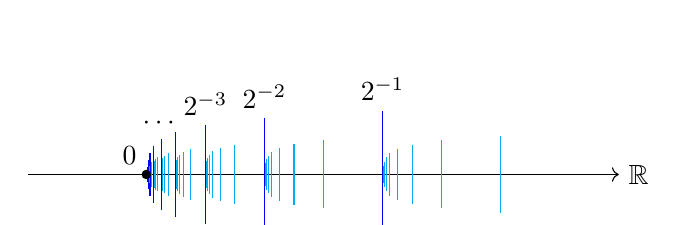
\begin{tikzpicture}[scale=6]
        \draw[->] (-0.25,0) -- (1,0) node[right] {$\mathbb{R}$};
        \foreach \n in {1,...,10} {
            \foreach \m in {1,...,10} {
                \draw[cyan, thin]
                    ({2^(-\n)+2^(-\n-\m)},{-0.1*((10-\n)/10)*((10-\m)/10)})
                 -- ({2^(-\n)+2^(-\n-\m)},{ 0.1*((10-\n)/10)*((10-\m)/10)});
            }
            \ifnum\n<4
                \draw[blue]
                    ({2^(-\n)},{-0.15*((10-\n)/10)})
                 -- ({2^(-\n)},{ 0.15*((10-\n)/10)})
                    node[black,above,scale=1] {$2^{-\n}$};
            \else
                \ifnum\n=5
                    \draw[blue]
                        ({2^(-\n)},{-0.15*((10-\n)/10)})
                     -- ({2^(-\n)},{ 0.15*((10-\n)/10)})
                        node[black,above,scale=1] {$\cdots$};
                \else
                    \draw[blue] 
                        ({2^(-\n)},{-0.15*((10-\n)/10)})
                     -- ({2^(-\n)},{ 0.15*((10-\n)/10)});
                \fi
            \fi
        }
        \filldraw (0,0) circle (0.25pt) node[above left] {$0$};
    \end{tikzpicture}
\end{center}

Simpler version without if/else clauses for labels:
\begin{center}
    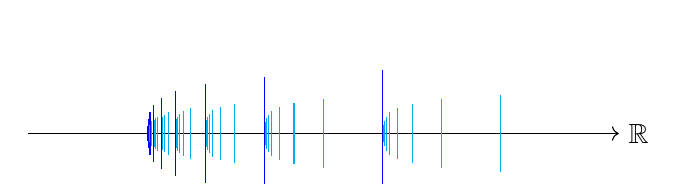
\begin{tikzpicture}[scale=6]
        \draw[->] (-0.25,0) -- (1,0) node[right] {$\mathbb{R}$};
        \foreach \n in {1,...,10} {
            \foreach \m in {1,...,10} {
                \draw[cyan, thin]
                    ({2^(-\n)+2^(-\n-\m)},{-0.1*((10-\n)/10)*((10-\m)/10)})
                 -- ({2^(-\n)+2^(-\n-\m)},{ 0.1*((10-\n)/10)*((10-\m)/10)});
            }
            \draw[blue]
                ({2^(-\n)},{-0.15*((10-\n)/10)})
             -- ({2^(-\n)},{0.15*((10-\n)/10)});
        }
    \end{tikzpicture}
\end{center}



\subsection*{Calc Library}

\begin{center}
    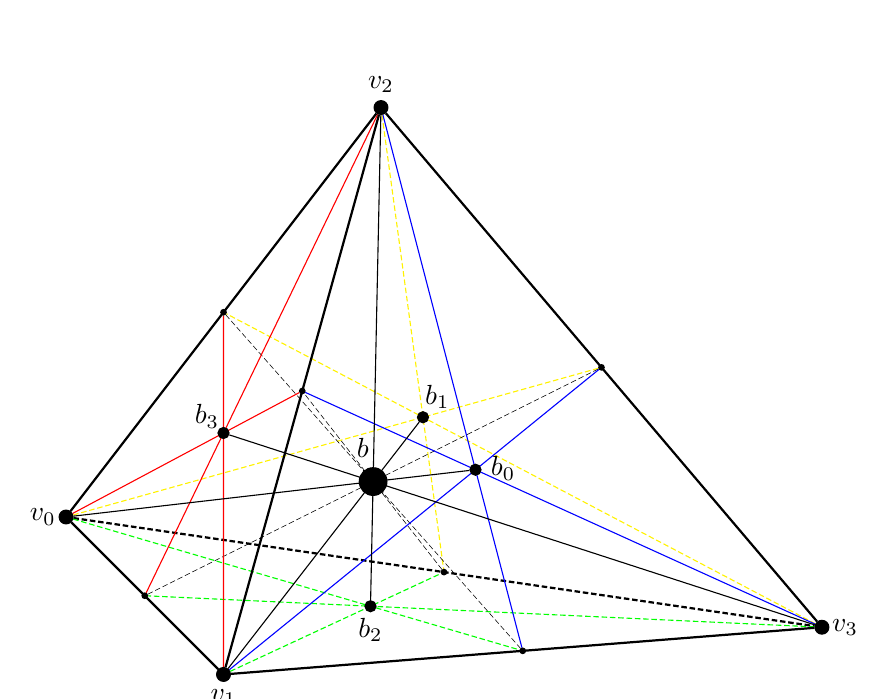
\begin{tikzpicture}[scale = 2]
        \begin{scope}[every node/.style={circle, fill, draw, inner sep=0, minimum size=5pt}]
            \node[label=left:{$v_0$}]  (v0) at (0,1) {};
            \node[label=below:{$v_1$}] (v1) at (1,0) {};
            \node[label=above:{$v_2$}] (v2) at (2,3.6) {};
            \node[label=right:{$v_3$}] (v3) at (4.8,0.3) {};
        \end{scope}
        \begin{scope}[every node/.style={circle, fill, draw, inner sep=0, minimum size=2pt}]
            \node (b01) at ($ 1/2*(v0) + 1/2*(v1) $) {};
            \node (b02) at ($ 1/2*(v0) + 1/2*(v2) $) {};
            \node (b03) at ($ 1/2*(v0) + 1/2*(v3) $) {};
            \node (b12) at ($ 1/2*(v1) + 1/2*(v2) $) {};
            \node (b13) at ($ 1/2*(v1) + 1/2*(v3) $) {};
            \node (b23) at ($ 1/2*(v2) + 1/2*(v3) $) {};
        \end{scope}
        \begin{scope}[every node/.style={circle, fill, draw, inner sep=0, minimum size=4pt}]
            \node[label={[xshift=1.5pt,yshift=0.5pt]0:{$b_0$}}]
                (b0) at ($ 1/3*(b13) + 1/3*(b12) + 1/3*(b23) $) {};
            \node[label={[yshift=1pt]70:{$b_1$}}]
                (b1) at ($ 1/3*(b02) + 1/3*(b03) + 1/3*(b23) $) {};
            \node[label=below:{$b_2$}]
                (b2) at ($ 1/3*(b01) + 1/3*(b03) + 1/3*(b13) $) {};
            \node[label=above left:{$b_3$}]
                (b3) at ($ 1/3*(b01) + 1/3*(b02) + 1/3*(b12) $) {};
        \end{scope}
        \begin{scope}[on background layer]
            \draw[thick, dash pattern=on 2pt off 1pt]
                (v0) -- (v3);
            \draw[yellow, dash pattern=on 2pt off 1pt]
                (v0) -- (b23)
                (v2) -- (b03)
                (v3) -- (b02);
            \draw[green, dash pattern=on 2pt off 1pt]
                (v0) -- (b13)
                (v1) -- (b03)
                (v3) -- (b01);
            \draw[very thin, dash pattern=on 2pt off 1pt]
                (b01) -- (b23)
                (b02) -- (b13)
                (b03) -- (b12);
            \draw[red]
                (v0) -- (b12)
                (v1) -- (b02)
                (v2) -- (b01);
            \draw[blue]
                (v1) -- (b23)
                (v2) -- (b13)
                (v3) -- (b12);
            \draw
                (v0) -- (b0)
                (v1) -- (b1)
                (v2) -- (b2)
                (v3) -- (b3);
            \draw[thick]
                (v0) -- (v1)
                (v0) -- (v2)
                (v1) -- (v2)
                (v1) -- (v3)
                (v2) -- (v3)
                (v2) -- (v3);
        \end{scope}
        \filldraw
            ($ 1/8*(v0) + 1/8*(v1) + 1/8*(v2) + 1/8*(v3)
             + 1/8*(b0) + 1/8*(b1) + 1/8*(b2) + 1/8*(b3) $)
            circle (2.5pt) node [above left=5pt and -2pt] {$b$};
    \end{tikzpicture}
\end{center}



\section*{Exercises}

Time to put everything together. Recreate the following diagram:

\begin{center}
    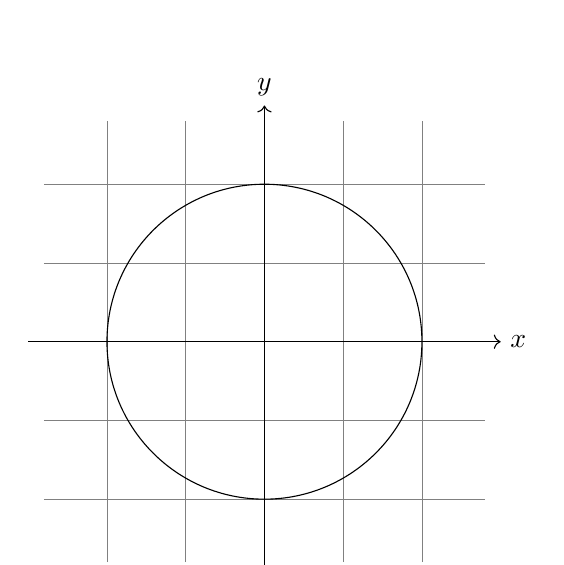
\begin{tikzpicture}[scale=2]
        \draw[step=.5,help lines] (-1.4,-1.4) grid (1.4,1.4);
        \draw[->] (-1.5,0) -- (1.5,0) node [right] {$x$};
        \draw[->] (0,-1.5) -- (0,1.5) node [above] {$y$};
        \draw (0,0) circle (1cm);
    \end{tikzpicture}
\end{center}








\end{document}